\chapter{Experiments And Results}\label{chp:experiments-and-results}
	
%\section{Experiments and Results}
% Ablation studies
% Problem with "global" pose -> incremental pose
% Training
%	- Different learning rate for pretrained flownet
%	- Dropout Regularization
	This chapter presents all experiments conducted on the deep learning model that was introduced in chapter~\ref{chp:the_model}.
	The results shown here give useful insights that supplement the work of \cite{wang2017deepvo}.
	\todo{table with default values}
	
	\section{Dataset Size and Dropout}
		We start by training the proposed model on the KITTI dataset on small subsequences of 25 frames. 
		Initially, the sequences are divided without overlap, that is, each video frame is part of exactly one subsequence.
		In addition, to simulate a dataset with more subsequences, the overlap is set to 20 frames (80\%). 
		This means that for each subsequence there is another one that differs by 5 frames.
		Table~\ref{tbl:kitti-overlap-and-dropout} compares the test error for models trained with and without overlap.
		\begin{table}[tb]
			\small
			\begin{center}
				\begin{tabular}{ccccrrr}
					\toprule
					\multicolumn{3}{c}{\textbf{Experiments}}	&	& \multicolumn{3}{c}{\textbf{Test error}} 		\\
					\cmidrule(lr){1-3} 					\cmidrule(lr){5-7}
					Length 			& Overlap 	& Dropout	&	& Total 	& Rotation	& Translation	\\ 
					\midrule
					25				& 0			& 0			& 	& 19.0293	& 0.4981	& 18.5312		\\ 
					25				& 20		& 0			&	& 16.5471	& 0.3913	& 16.1558		\\ 
					100				& 20		& 0			&	& 529.9459	& 39.8967	& 490.0493		\\ 
					100				& 80		& 0			& 	& 313.1278	& 47.8437	& 265.2841		\\ 
					100 			& 5			& 0.5		&	& 376.7666	& 43.1578	& 333.6088		\\ 
					%$20\rightarrow120$ 	& 5		& 0.5		&	& 303.7696	& 39.4114	& 264.3582		\\
					$20\rightarrow100$ 	& 5		& 0.5		&	& 289.8579 	& 42.0427 	& 247.8152 		\\
					\bottomrule
				\end{tabular}
			\end{center}
			\caption[Experiments on KITTI: Overlap and dropout]
					{Experiments on KITTI: Overlap and dropout. 
					 Shown is the test error on sequence 10 for different overlap and dropout during training.
					 The evaluation on the test set is performed on sequences of the same size as seen during training, and without overlap.
					 In the last row, the sequence length grows by one frame every epoch.
					 Each model was trained with default parameters for 100 epochs, except the last one which was trained for only 80 epochs.
					 \label{tbl:kitti-overlap-and-dropout}}
		\end{table}
		After the same number of epochs, the test error is about 13\% lower for the model trained on overlapping sequences with a decrease of 21\% for rotation and 12\% for translation.
		The same experiment is repeated by training on sequences of 100 frames with overlap 20 vs. overlap 80. 
		% Total error decreases by about 40\%.
		The translation error decreases by almost 46\%, however, the rotation loss increases.
		A similar observation can be made when using dropout on the LSTM output (before the fully-connected layer), as seen in the second last row of table~\ref{tbl:kitti-overlap-and-dropout}.
		
		For the last experiment in table~\ref{tbl:kitti-overlap-and-dropout}, the sequence length grows by an increment of one frame every epoch, starting from 20 frames and stopping at 100 frames after 80 epochs.
		As we can see, this method of training in combination with the dropout gives the best overall loss on the test set.
		A possible explanation for this could be the that the learning process is faster for short sequences because the LSTM requires a less complex memory mapping in order to remember the coordinate transforms from earlier time steps, including the first one.
		A gradual refinement of such a mapping may be less challenging for the optimization as opposed to learning it directly from long sequences.
		\todo{Need more explanation here.}
		
		Although the numbers in the table can be used to compare the different experiments, they are not very insightful by themselves.
		From the sum of squared differences alone, it is not possible to understand how the error behaves across the sequence.
		For better visualization, we can compute the error at regular distance intervals along the estimated path.
		Figure~\ref{fig:kitti-avg-rotation-translation-error-vs-path-distance} shows translation and rotation errors for path distance on subsequences of the KITTI sequence 10.
		\begin{figure}[t]
			\centering
			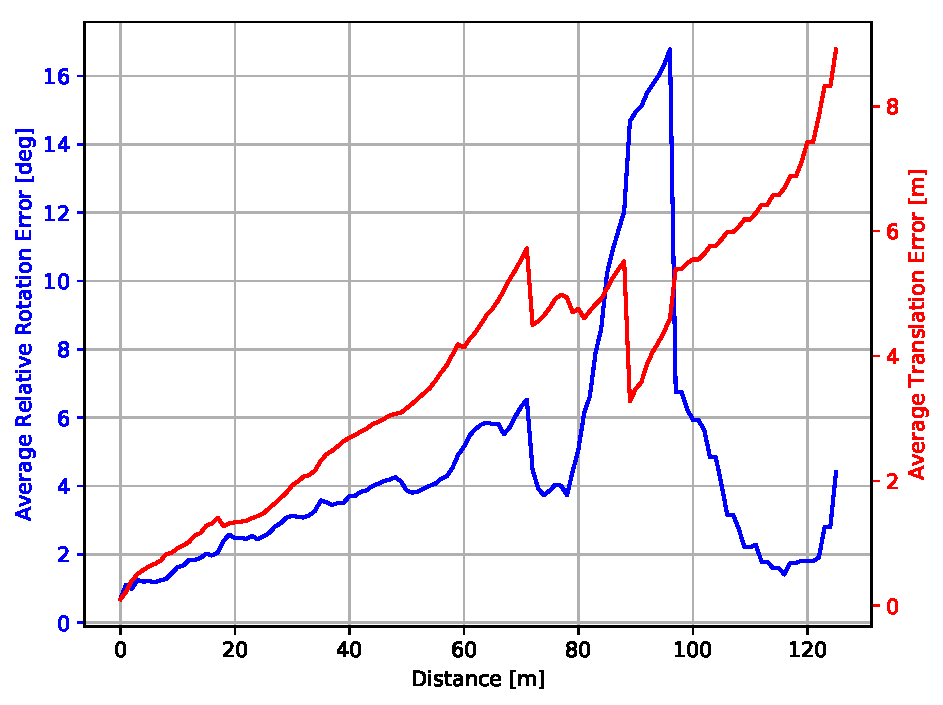
\includegraphics[width=0.5\linewidth]{Python-Plots/deepvo-KITTI/relative-rotation-and-translation-error-along-path-overlap80}
			\caption[Experiments on KITTI: Average rotation- and translation error vs. path distance]
					{Experiments on KITTI: Average rotation- and translation error vs. path distance.
					 The relative rotation- and translation error is evaluated at equal intervals along the subsequences of KITTI sequence 10.
					 The errors at the same distance are averaged over all sequences of that length.
					 \label{fig:kitti-avg-rotation-translation-error-vs-path-distance}}
		\end{figure}
		The relative rotation error is the angle of rotation around the axis corresponding to the relative rotation between estimated- and ground truth pose.
		\todo{refer to equations introduced in previous chapter}
		
		\paragraph{Discussion}
		From these experiments, we can conclude that sequence overlap and dropout have a positive impact on the generalization of translation estimates.
		Especially when training data is scarce, the overlap method can be utilized to artificially increase the dataset and reduce the error on the test data.
		
	\section{The Problem on Long Sequences}
		In the experiments before, the model was always tested on subsequences with the same length as during training.
		However, in a real-world application, we would like to test the model on sequences with an arbitrary number of frames, and potentially the test sequences are much longer than the ones seen during training.
		Table~\ref{tbl:kitti-testing-on-longer-sequences} shows an experiment where the sequence length between training set and test set changes.
		\begin{table}[tb]
			\small
			\begin{center}
				\begin{tabular}{cccrrr}
					\toprule
					\multicolumn{2}{c}{\textbf{\#Frames}}	&	& \multicolumn{3}{c}{\textbf{Test error}} \\ 
					\cmidrule(lr){1-2} 									\cmidrule(lr){4-6}
					Training 		& Test 			&	& Total 	& Rotation	& Translation	\\ 
					\midrule
					25				& 25			&	& 16.5471	& 0.3913	& 16.1558		\\
					25				& 100			&	& 1060.7528	& 37.6196	& 1023.1332		\\
					100				& 100			&	& 529.9459	& 39.8967	& 490.0493		\\ 
					\bottomrule
				\end{tabular}
			\end{center}
			\caption[Experiments on KITTI: Testing on longer sequences]
					{Experiments on KITTI: Testing on longer sequences. 
					 When testing on sequences with more frames, the error becomes extremely high compared to the model trained on 100 frames.
				 \label{tbl:kitti-testing-on-longer-sequences}}
		\end{table}
		The problem: The model trained on sequences with 25 frames does not generalize to sequences of 100 frames.
		This is a very undesired result, after all, the recurrent part of the network was designed with the intention to handle arbitrary input sizes.
		From the results in table~\ref{tbl:kitti-testing-on-longer-sequences} it appears that the network is able to memorize the sequence length and therefore overfits to the specific length it is trained on.
		The attempt to counteract this behavior with sequences of random size failed.
		The network would still overfit to the average length of sequences seen during training.
		Figure~\ref{fig:kitti-testing-on-longer-sequences} visualizes the camera path on a test sequence of 100 frames.
		\begin{figure}
			\centering
			\begin{subfigure}[b]{0.5\linewidth}
				\centering
				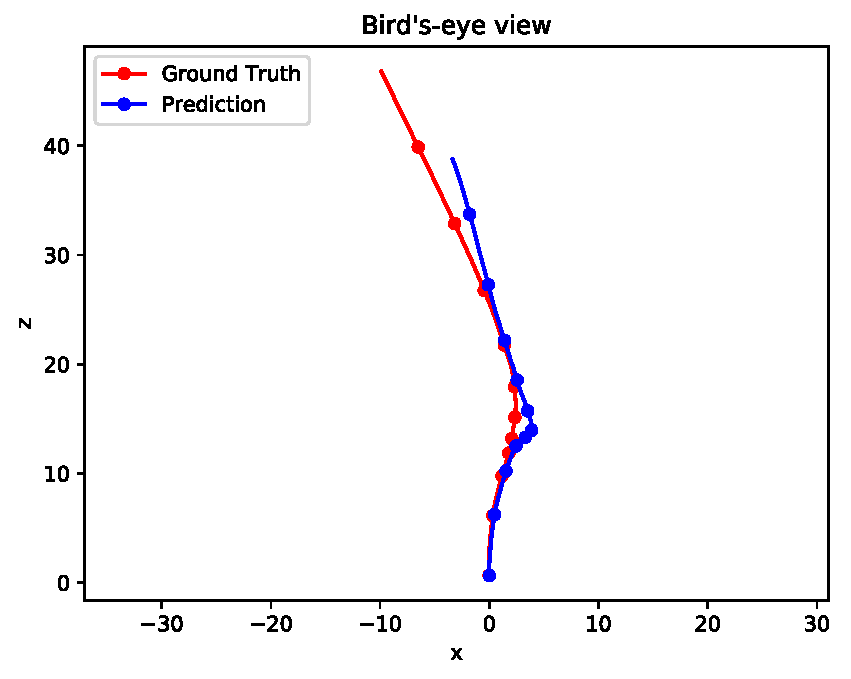
\includegraphics[width=\linewidth]{Experiments/trained-on-25-frames}
				\caption{
					\label{fig:0}
				}
			\end{subfigure}%
			\begin{subfigure}[b]{0.5\linewidth}
				\centering
				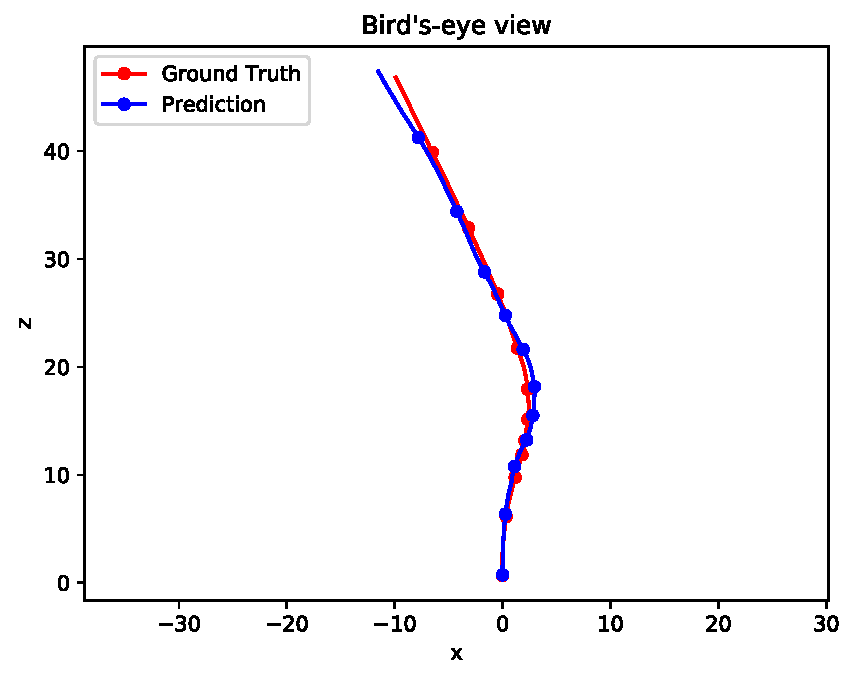
\includegraphics[width=\linewidth]{Experiments/trained-on-100-frames}
				\caption{
					\label{fig:1}
				}
			\end{subfigure}%
			\caption[Training and testing on different sequence length]
					{Training and testing on different sequence length. 
					 Two models tested on a KITTI subsequence of 100 frames when trained on sequences of (a) 25 frames and (b) 100 frames. 
					 The markers in the plot are shown every ten frames.
					 The scale of the axes is in meters.
					 \label{fig:kitti-testing-on-longer-sequences}}
		\end{figure}
		One can observe that the estimated path quickly diverges after 25 frames.
		However, when trained on sequences with 100 frames, the estimation is more accurate.
		
		\paragraph{Discussion}
		The experiments in this section reveal a serious problem.
		One of the main purposes of the LSTM is to handle arbitrary input length, and yet, in the scenario we have so far it is not able to do so.
		In the general application of VO, it is not realistic to assume a maximum length for a video and to train the model only for that length.
		
		
	\section{Training with Incremental Poses}
		One potential reason for why the model is overfitting to a certain length could be semantic difference between input and output.
		Since input at each time step is a pair of consecutive images in the video, the observed motion (by the LSTM) is relative to the current time step.
		On the other hand, the output pose is forced to be in the global coordinate system given by the very first video frame.
		This difference could potentially cause confusion and lead to the overfitting problem.
		
		To address the issue, we convert the ground truth poses to incremental poses using the formula from equation~\ref{eq:relative_rotation_conversion_general} by setting $j = i - 1$.
		The first two rows of table~\ref{tbl:kitti-incremental-pose-and-lstm-removal} show the results of training with incremental pose.
		At test time, the output poses are converted back into the global coordinate system for evaluating the loss on the test set.
		This allows for a direct comparison with the previous results from table~\ref{tbl:kitti-testing-on-longer-sequences}.
		\begin{table}[tb]
			\small
			\begin{center}
				\begin{tabular}{cccccrrr}
					\toprule
					\multicolumn{5}{c}{\textbf{Experiments}}		& \multicolumn{3}{c}{\textbf{Test error}} 		\\
					\cmidrule(lr){1-4} 	\cmidrule(lr){6-8}
					\multicolumn{2}{c}{Length} & Dropout & LSTM &	& Total & Rotation & Translation	\\ 
					Training & Test & & & & & & \\
					\midrule
					25 & 25		& 0			& \cmark 	& 	& 22.0498	& 0.5642	& 21.4856 		\\ 
					25 & 25		& 0.5		& \cmark 	& 	& 21.0171	& 0.4957	& 20.5214		\\ 
					25 & 25		& 0			& \xmark 	& 	& 22.4305	& 0.5121	& 21.9184		\\ 
					25 & 100	& 0			& \cmark 	& 	& 335.5754	& 16.5476	& 319.0277 		\\ 
					25 & 100	& 0.5		& \cmark 	& 	& 301.5090	& 22.9736	& 278.5354 		\\ 
					25 & 100	& 0			& \xmark 	& 	& 378.8834	& 48.4604	& 330.4230 		\\ 
					\bottomrule
				\end{tabular}
			\end{center}
			\caption[Experiments on KITTI: Training with incremental poses]
					{Experiments on KITTI: Training with incremental poses.
					 Three variants are tested: LSTM, LSTM with dropout layer, and LSTM replaced with fully-connected layer.
					 Shown is the loss on the test set with incremental poses converted to global poses.
					 \label{tbl:kitti-incremental-pose-and-lstm-removal}}
		\end{table}
		From these results we can see that the error is significantly lower when testing on long sequences.
		Since the only difference in the experiments is the format of the pose, it can be concluded that training with incremental pose is the preferred way.
		In the paper of \cite{wang2017deepvo}, it is never explicitly stated which coordinate system is used.
		The results in this thesis suggest that \citeauthor{wang2017deepvo} have also used incremental poses in their experiments.
		
		The new approach of training the network with incremental poses raises an important question.
		What exactly is the contribution of the LSTM?
		Since the pose is not global anymore, the LSTM is not forced to keep track of the accumulation of pose changes from the past frames.
		To investigate this question, we conduct an experiment where the LSTM is replaced with a fully-connected layer followed by a ReLU.
		The previous affine output layer is kept, making it a total of two affine layers that regress the pose from the CNN features.
		This eliminates the recurrence from the network, and all pose estimations are performed solely on consecutive frames.
		Each output is independent of the previous inputs, therefore it is simply a feedforward network.
		The last row of table~\ref{tbl:kitti-incremental-pose-and-lstm-removal} shows a higher loss on the test set when using the replacement.
		This would suggest that the recurrence does indeed result in a better VO performance.
		However, when looking at the rotation and translation error along the path in figure~\ref{fig:avg-rotation-and-translation-error-dropout-no-LSTM} (blue), and compare it with the version that uses the LSTM (red, green), the error is actually lower for most of the path.
		\begin{figure}
			\centering
			\begin{subfigure}[b]{0.5\linewidth}
				\centering
				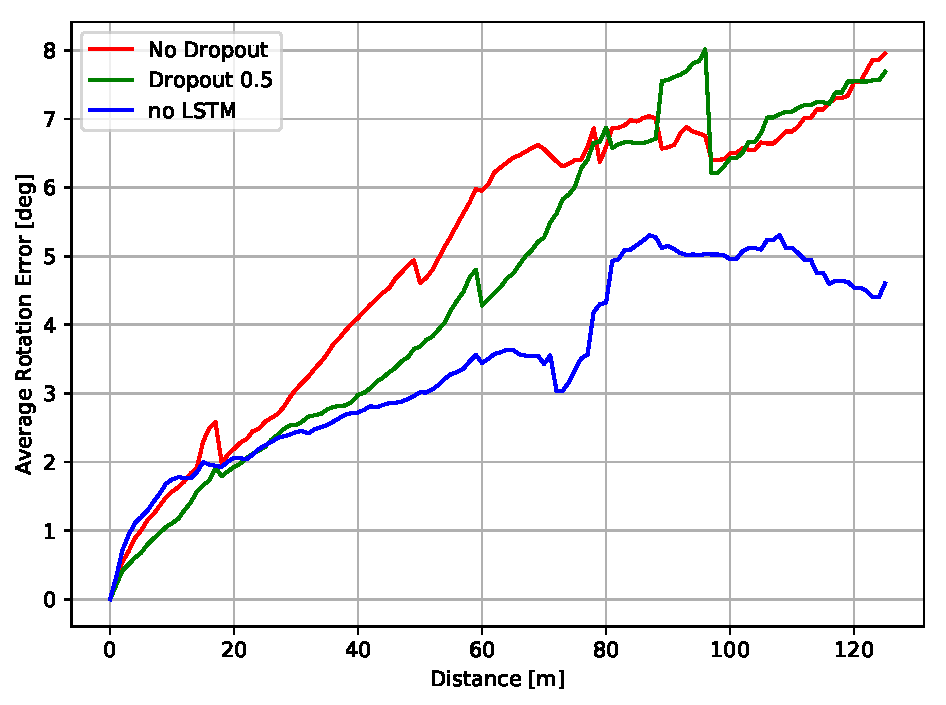
\includegraphics[width=\linewidth]{Python-Plots/deepvo-KITTI/rotation-error-per-meter-comparison-Dropout-No-LSTM}
				\caption{
					Rotation
					\label{fig:avg-rotation-error-dropout-no-LSTM}
				}
			\end{subfigure}%
			\begin{subfigure}[b]{0.5\linewidth}
				\centering
				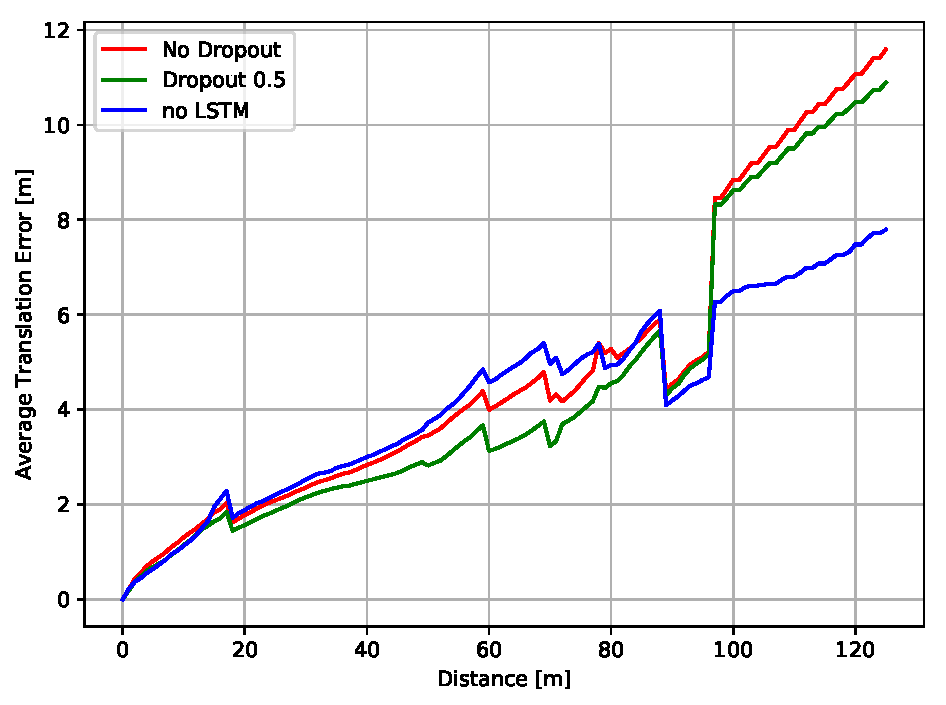
\includegraphics[width=\linewidth]{Python-Plots/deepvo-KITTI/translation-error-per-meter-comparison-Dropout-No-LSTM}
				\caption{
					Translation
					\label{fig:avg-translation-error-dropout-no-LSTM}
				}
			\end{subfigure}%
			\caption[Comparison: LSTM vs. LSTM with dropout vs. no LSTM]
					{Comparison of the rotation and translation error on subsequences of KITTI sequence 10 for three different models:
					 LSTM, LSTM with dropout, and LSTM replaced with fully-connected layer.
					 \label{fig:avg-rotation-and-translation-error-dropout-no-LSTM}}
		\end{figure}
		In addition, figure~\ref{fig:kitti-test-sequence-10-lstm-vs-no-lstm} shows the predicted path of the full KITTI sequence 10.
		Although the shape of the two paths is roughly the same, the feedforward model is closer to the ground truth path, experiencing smaller translational drift.
		\begin{figure}
			\centering
			\begin{subfigure}[b]{0.5\linewidth}
				\centering
				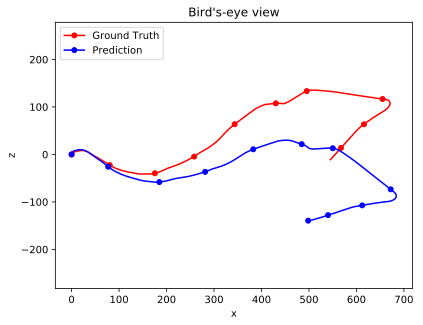
\includegraphics[width=\linewidth]{Experiments/lstm-vs-fc/incremental-dropout-lstm}
				\caption{
					LSTM
					\label{fig:kitti-sequence-10-lstm}
				}
			\end{subfigure}%
			\begin{subfigure}[b]{0.5\linewidth}
				\centering
				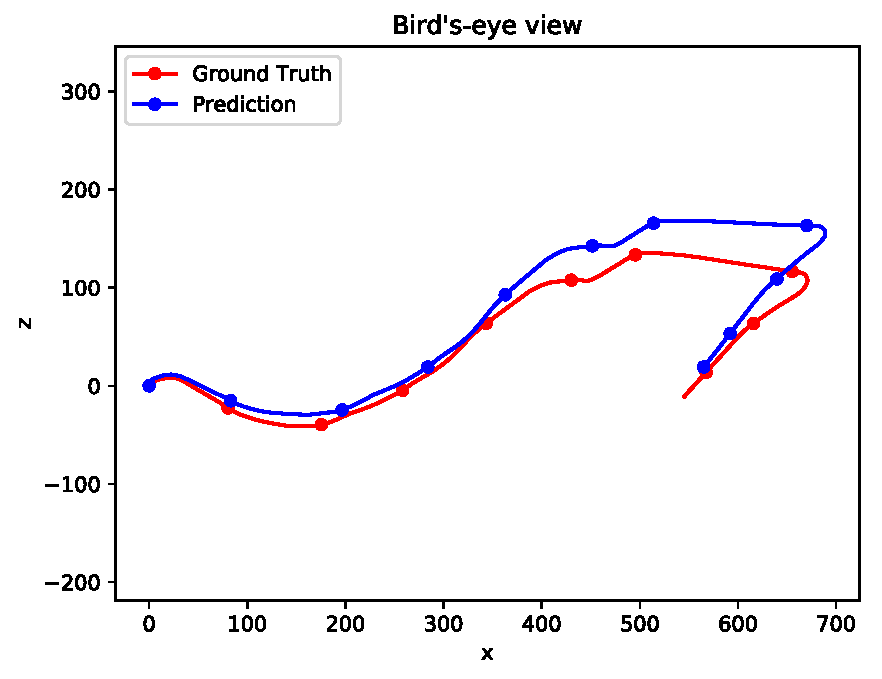
\includegraphics[width=\linewidth]{Experiments/lstm-vs-fc/incremental-dropout-no-lstm}
				\caption{
					Feedforward
					\label{fig:fig:kitti-sequence-10-no-lstm}
				}
			\end{subfigure}%
			\caption[Estimated motion on KITTI test sequence 10: LSTM vs. feedforward network]
					{Estimated motion on KITTI test sequence 10: LSTM (a) vs. feedforward network (b).
					 The estimated incremental poses are converted to global poses in order to recreate the path.
					 The coordinate axes are in meters, and a marker is plotted every 120 frames.
					 \label{fig:kitti-test-sequence-10-lstm-vs-no-lstm}}
		\end{figure}
		
		\paragraph{Discussion}
		In this second set of experiments, we have addressed the issue where the LSTM would overfit to a certain number of frames seen during training.
		When forced to output incremental poses, the model is able to estimate motion from videos of arbitrary sizes.
		However, it is still unclear if and to what amount the LSTM uses the hidden state that encodes the past.
		In fact, as we have shown, a feedforward network (without recurrence) is able to outperform the LSTM.
		Based on these observations, one might speculate that the recurrent connection hurts the performance.
		But this is not a very plausible, because during the optimization process the LSTM would learn to ignore the hidden state by setting the parameters of the cell gates accordingly, if this minimizes the loss.
		It is possible that the loss function in equation~\ref{eq:euler_pose_loss_function_t}, a balance between euclidean error of translation and rotation, is not well-suited for VO.
		\todo{continue: euler angles -- quaterions?}
		\begin{table}[tb]
			\small
			\begin{center}
				\begin{tabular}{lcrrrr}
					\toprule
					%\multicolumn{2}{c}{\textbf{Experiments}}		& \multicolumn{4}{c}{\textbf{Test error}} 		\\
					%\cmidrule(lr){1-2} 	\cmidrule(lr){3-6}
					\textbf{Hidden state} & & \multicolumn{2}{c}{\textbf{Relative Pose}} & \multicolumn{2}{c}{\textbf{Global Pose}} \\
					& & Rotation & Translation & Rotation & Translation \\
					\midrule
					Reset 		& 			& 0.2319	& 5.7220	& 9.8600	& 262.7984		\\ 
					Keep		&			& 0.3097	& 8.5461	& 12.7551	& 426.7877		\\
					\bottomrule
				\end{tabular}
			\end{center}
			\caption[Experiments on VIPER: Carrying over the hidden state vs. resetting it]
					{Experiments on VIPER: Carrying over the hidden state vs. resetting it.
					 \label{tbl:kitti-removing-lstm}}
		\end{table}
	
		\begin{figure}[t]
			\centering
			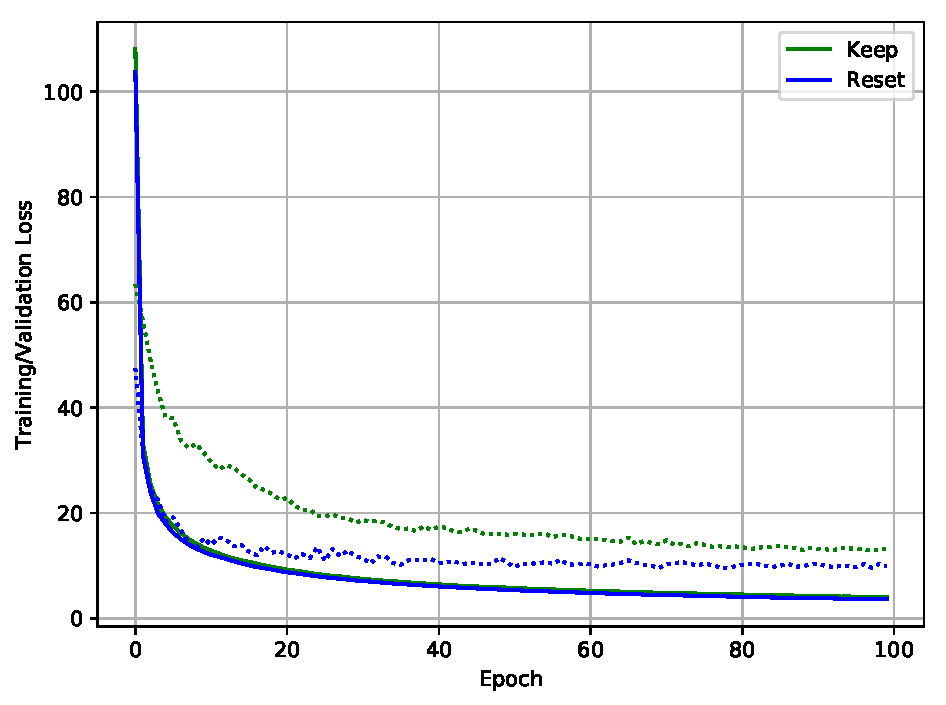
\includegraphics[width=0.7\linewidth]{Python-Plots/deepvo-VIPER/convergence-speed-keep-vs-reset}
			\caption[]
					{Convergence speed comparison state reset vs. keep.}
		\end{figure}
		
		\subsection{Euler Angles vs. Quaternions}
		
			\begin{figure}
				\centering
				\begin{subfigure}[b]{0.5\linewidth}
					\centering
					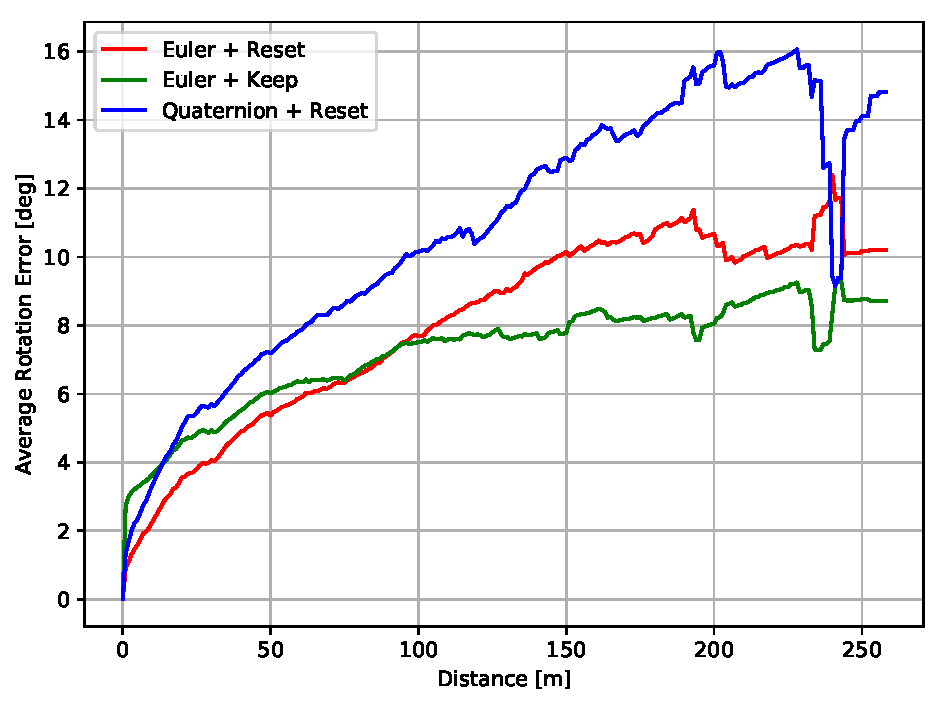
\includegraphics[width=\linewidth]{Python-Plots/deepvo-VIPER/rotation-comparison-Euler-Quaternion-Reset-or-Keep-Hidden}
					\caption{}
				\end{subfigure}%
				\begin{subfigure}[b]{0.5\linewidth}
					\centering
					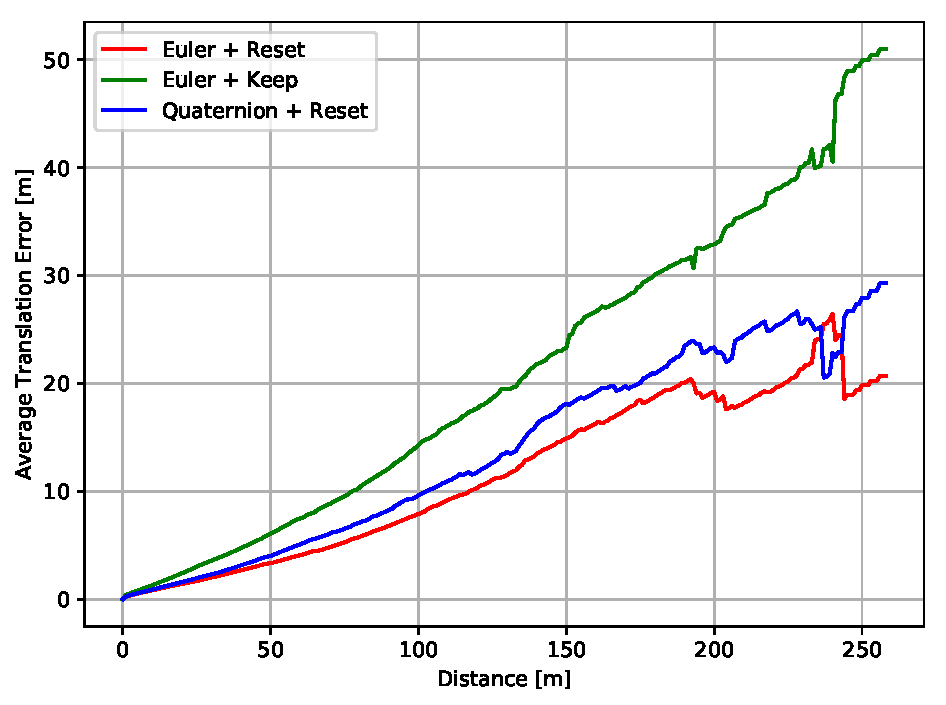
\includegraphics[width=\linewidth]{Python-Plots/deepvo-VIPER/translation-comparison-Euler-Quaternion-Reset-or-Keep-Hidden}
					\caption{}
				\end{subfigure}%
				\caption[Experiments on VIPER: Euler vs. quaternion vs. hidden state transfer]
						{Experiments on VIPER: Euler vs. quaternion vs. hidden state transfer.
						 50 epochs, 100 frames, no dropout, shuffling for reset
						 \label{fig:viper-euler-vs-quat-vs-hidden-state-keep-or-reset}}
			\end{figure}
		

		\begin{figure}
			\centering
			\begin{subfigure}[b]{\linewidth}
				\centering
				\includegraphics[width=0.45\linewidth]{example-image-a}
				\includegraphics[width=0.45\linewidth]{example-image-a}
				\caption{
					Long, curve
					\label{fig:0}
				}
			\end{subfigure}%
			\\
			\begin{subfigure}[b]{\linewidth}
				\centering
				\includegraphics[width=0.45\linewidth]{example-image-b}
				\includegraphics[width=0.45\linewidth]{example-image-b}
				\caption{
					Short
					\label{fig:0}
				}
			\end{subfigure}%
			\\
			\begin{subfigure}[b]{\linewidth}
				\centering
				\includegraphics[width=0.45\linewidth]{example-image-c}
				\includegraphics[width=0.45\linewidth]{example-image-c}
				\caption{
					\label{fig:0}
				}
			\end{subfigure}%
			\caption[Qualitative results for motion estimation on KITTI]
					{Qualitative results for motion estimation on KITTI.
				 Left column: Visualization of the estimated and true path.
				 Right column: Plot of each coordinate axis.
				 Markers are shown for every \todo{xx} frames.
					\label{fig:0}}
		\end{figure}


		\begin{figure}
			\centering
			\begin{subfigure}[b]{\linewidth}
				\centering
				\includegraphics[width=0.45\linewidth]{example-image-a}
				\includegraphics[width=0.45\linewidth]{example-image-a}
				\caption{
					Long, curve
					\label{fig:0}
				}
			\end{subfigure}%
			\\
			\begin{subfigure}[b]{\linewidth}
				\centering
				\includegraphics[width=0.45\linewidth]{example-image-b}
				\includegraphics[width=0.45\linewidth]{example-image-b}
				\caption{
					Short
					\label{fig:0}
				}
			\end{subfigure}%
			\\
			\begin{subfigure}[b]{\linewidth}
				\centering
				\includegraphics[width=0.45\linewidth]{example-image-c}
				\includegraphics[width=0.45\linewidth]{example-image-c}
				\caption{
					\label{fig:0}
				}
			\end{subfigure}%
			\caption[Qualitative results for motion estimation on VIPER]
					{Qualitative results for motion estimation on VIPER.
				 \label{fig:0}}
		\end{figure}